%%%%%
%%%%%  Naudokite LUALATEX, ne LATEX.
%%%%%
%%%%
\documentclass[]{VUMIFTemplateClass}

\usepackage{indentfirst}
\usepackage{amsmath, amsthm, amssymb, amsfonts}
\usepackage{mathtools}
\usepackage{physics}
\usepackage{graphicx}
\usepackage{verbatim}
\usepackage[hidelinks]{hyperref}
\usepackage{color,algorithm,algorithmic}
\usepackage[nottoc]{tocbibind}
\usepackage{tocloft}

\usepackage{titlesec}
\newcommand{\sectionbreak}{\clearpage}

\makeatletter
\renewcommand{\fnum@algorithm}{\thealgorithm}
\makeatother
\renewcommand\thealgorithm{\arabic{algorithm} algoritmas}

\usepackage{biblatex}
\bibliography{bibliografija}
%% norint pakeisti bibliografijos šaltinių numeravimą (skaitiniu arba raidiniu), pakeitimus atlikti VUMIFTemplateClass.cls 150 eilutėje

% Author's MACROS
\newcommand{\EE}{\mathbb{E}\,} % Mean
\newcommand{\ee}{{\mathrm e}}  % nice exponent
\newcommand{\RR}{\mathbb{R}}


\studijuprograma{\{Studijų programos\}} %Studijų programą įrašyti kilmininko linksniu (pavyzdžiui – Programų sistemų, Finansų ir draudimų matematikos ir t. t.)
\darbotipas{\{Darbo tipas\}} % Bakalauro baigiamasis darbas arba magistro baigiamasis darbas
\darbopavadinimas{Darbo pavadinimas lietuvių kalba}
\darbopavadinimasantras{Work Title in English}
\autorius{Vardas Pavardė}

%Autorių gali būti ir daugiau, tuo atveju, kiekvienas autorius rašomas iš naujos eilutės, ir pridedamas titulinis.tex arba dvigubasTitulinis.tex dokumentuose
%\antrasautorius{Vardas Pavardė} %Jei toks yra, kitu atveju ištrinti

\vadovas{pedagoginis/mokslinis vardas Vardas Pavardė}
\recenzentas{pedagoginis/mokslinis vardas Vardas Pavardė} %Jei toks yra žinomas, kitu atveju ištrinti
\moksliniskonsultantas{pedagoginis/mokslinis vardas Vardas Pavardė} %Jei toks yra žinomas, kitu atveju ištrinti

\begin{document}
\selectlanguage{lithuanian}

\onehalfspacing
\begin{titlepage}
\vskip 20pt
\begin{center}

\includegraphics[scale=0.55]{images/MIF.png}
\end{center}

\makeatletter

\vskip 20pt
\centerline{\bf \large \textbf{VILNIAUS UNIVERSITETAS}}
\vskip 10pt
\centerline{\large \textbf{MATEMATIKOS IR INFORMATIKOS FAKULTETAS}}
\vskip 10pt
\centerline{\large \textbf{\MakeUppercase{\@studijuprograma \space studijų programa}}}

\vskip 80pt
\centerline{\Large \@darbotipas}
\vskip 20pt
\begin{center}
    {\bf \LARGE \@darbopavadinimas}
\end{center}
\begin{center}
    {\bf \Large \@darbopavadinimasantras}
\end{center}
\vskip 80pt

\centering{\Large \@autorius}
\@ifundefined{@antrasautorius}{}
{
\vskip 10pt
\centering{\Large \@antrasautorius}
}
\vskip 20pt

\centering{
    \begin{tabular}{rcp{.7\textwidth}}
        {\Large Darbo vadovas} & {\Large :} & {\Large \@vadovas}\\[10pt]
        \@ifundefined{@moksliniskonsultantas}{}
            {
                {\Large Mokslinis konsultantas} & {\Large :} & {\Large \@moksliniskonsultantas}\\[10pt]
            }
        \@ifundefined{@recenzentas}{}
            {
                {\Large Recenzentas} & {\Large :} & {\Large \@recenzentas}\\[10pt]
            }
    \end{tabular}}


\vskip 110pt

\centerline{\large \textbf{Vilnius}}
\centerline{\large \textbf{\the\year{}}}

\makeatother

\newpage
\end{titlepage}
%\newgeometry{top=2cm,bottom=2cm,right=2cm,left=3cm}
\setcounter{page}{2}


%% Padėkų skyrius
\sectionnonumnocontent{Padėka}
Darbo autorius dėkoja Vilniaus universiteto Matematikos ir informatikos fakulteto Informacinių technologijų atviros prieigos centrui už suteiktus našiųjų skaičiavimų (angl. High Performance Computing, HPC) išteklius šio darbo tyrimui atlikti.
%%
%%
%%      Jei baigiamojo darbo tyrimui atlikti naudojote MIF suteikiamus IT išteklius (CPU-h, GPU-h, kitus IT resursus), padėką palikite, jei nenaudojote - galite ištrinti.
%%
%%

Čia taip pat galima pridėti padėkas įvairiems kitiems dalykams, pavyzdžiui: vadovui, universitetui, įmonei ir t. t.

%%Santrauka
\selectlanguage{lithuanian}
\sectionnonum{Santrauka}

Darbo santrauka.\\

\textbf{Raktiniai žodžiai:} čia surašomi su darbu susiję raktiniai žodžiai, \textit{\textbf{minimalus raktinių žodžių kiekis - 3}}, tačiau jų gali būti ir daugiau.


\sectionnonum{Summary}

Summary in english.\\

\textbf{Keywords:} work related keywords, with a \textit{\textbf{minimum of 3 keywords}}, but can be more.


\singlespacing

% iliustracijų sąrašas, jei jo nereikia - ištrinkite
\listoffigures 

%lentelių sąrašas, jei jo nereikia - ištrinkite
\listoftables

%Turinys
\tableofcontents
\onehalfspacing


%Žymėjimų skyrius
\sectionnonum{Žymėjimai}
Šis skyrius skirtas, jei yra naudojami žymėjimai. Pavyzdžiui:    
\begin{itemize}
    \item $\EE X$ žymi atsitiktinio dydžio $X$ vidurkį.
\end{itemize}
%Palikti jeigu reikia

%Sutrumpinimų skyrius
\sectionnonum{Santrumpos}
Šis skyrius skirtas, jei yra naudojamos santrumpos. Pavyzdžiui:

\begin{tabular}{rcp{.7\textwidth}}
    {v.p.n.a.d.} & {} & {vienodai pasiskirstę nepriklausomi atsitiktiniai dydžiai}
\end{tabular}
%Palikti jeigu reikia

\sectionnonum{Įvadas}
Bet kokiam rašto darbui rašyti būtina naudotis atitinkamos studijų programos metodiniais nurodymais\footnote{Visų programų naujausius metodinius reikalavimus galima rasti čia, atitinkamoje programoje: \url{https://mif.vu.lt/lt3/studijos/bakalaurams}}. Juose rasite visus rašto darbų nurodymus susijusius su citavimu, darbo struktūra, apimtimi ir t. t.


\section{Formatavimas}

Šiame skyriuje bus pateikti pavyzdžiai matematinio teksto, lentelių ir paveikslėlių formatavimams bei aprašyta, kaip taisyklingai suformuluoti matematinius jūsų baigiamojo darbo rezultatus.

\subsection{Matematinis tekstas}

Matematinės formulės gali būti įterptos teksto pastraipose, formulės \LaTeX~kodą atskiriant simboliais \texttt{\$...\$}. Pavyzdys: trigonometrinė tapatybė $\sin^2 \alpha + \cos^2 \alpha = 1$.

Tačiau formulės atrodys daug gražiau, jeigu jos bus išskirtos į atskiras lygtis, formulės kodą patalpinant į aplinką \texttt{\textbackslash[...\textbackslash]}. Štai tokios lygties pavyzdys:
\[
\ee^{i \alpha} = \cos{\alpha} + i \sin{\alpha}, \qquad \alpha \in \RR.
\]
Šioje lygtyje buvo panaudoti matematiniai simboliai $\RR$ ir $\ee$, kurių komandos \texttt{\textbackslash RR} ir \texttt{\textbackslash ee} apibrėžtos šablono pradžioje.

Kartais formulės užima kelias eilutes, pvz.:
\begin{equation}
\begin{split}
2&= 1+1+0=\left(\frac{\sqrt{16}}{\tan^2\pi/3+1}\right) +\ln\ee+\sin\pi\\
&= (\sin^2 17+\cos^2 17)^{\ln\ee}+\cos 0 +(x^{1/\ln x})'. 
\label{form1}
\end{split}
\end{equation}

Nepamirškite padėti taško ($.$) formulės pabaigoje, jeigu tai sakinio pabaiga. Taip pat akreipkite dėmesį į skliaustų, kurių viduje stovi didelė trupmena \texttt{\textbackslash frac}, aukštį, kuris automatiškai reguliuojamas komandomis \texttt{\textbackslash left( ... \textbackslash right)} arba nurodomas komandomis \texttt{\textbackslash big}, \texttt{\textbackslash Big}, \texttt{\textbackslash bbig}.

\bigskip

Jeigu formulės prisireiktų vėliau, jos nereikia kiekvieną kartą perrašinėti iš naujo. Reikiamą formulę visada galima pacituoti su komandą \texttt{\textbackslash eqref}. Pavyzdžiui, aukščiau užrašyta formulė su numeriu cituojama taip: lygtis \eqref{form1}. Tam reikia komanda \texttt{\textbackslash  label} formulei priskirti laikiną pavadinimą, kurį \LaTeX~automatiškai pakeis į reikiamą numerį. Daugiau informacijos apie \LaTeX~matematinius simbolius, lygtis, matematines aplinkas ir komandas galima rasti šiame dokumente \cite{amsdoc}.

\bigskip

Pateiksime dar keletą formulių, kuriose naudojamos sudėtingesnės matematinės komandos. Matricos ir determinantai užrašomi naudojant LaTeX aplinkas \texttt{pmatrix} ir \texttt{vmatrix}:
\[
A= \begin{pmatrix}
    0 & 1\\
    2 & 3
\end{pmatrix}, \qquad
\det A =
\begin{vmatrix}
0 & 1\\
2 & 3    
\end{vmatrix} = 0 \cdot 3 - 1 \cdot 2 = -2.
\]
Sudėtingesnėms lygtims ir matricoms formatuoti labai praverčia paketo \texttt{mathtools} \cite{mtoolsdoc} komandomis. Paketas \texttt{mathtools} įtrauktas į darbo šabloną, todėl jo komandomis galima naudotis tiesiogiai.

Išvestinė užrašoma naudojant apostrofo simbolį (\texttt{'}), pavyzdžiui,
\[
(f(x)g(x))' = f'(x)g(x) + f(x)g'(x).
\]
Teiloro polinomas:
\[
p(x) = p(a) + p'(a)(x-a)+\frac{p''(a)}{2!}(x-a)^2 + ... + \frac{p^{(n)}}{n!}(x-a)^n.
\]
Paprastoms ir dalinėms išvestinėms, diferencialams, gradientams ir pan. užrašyti į darbo šabloną įtrauktos labai patogios komandos \texttt{\textbackslash dv} ir \texttt{\textbackslash pdv}, \texttt{\textbackslash dd}, \texttt{\textbackslash grad} iš \texttt{physics} paketo \cite{physdoc}:
\[
\dv{f}{x},  \qquad
\dv[2]{f}{x}, \qquad
\pdv{f}{x},  \qquad
\pdv[5]{f}{x} \qquad
\pdv{f}{x}{y}, \qquad
\dd{f}, \qquad
\grad{f}
\]

Integralą su rėžiais užrašysime naudodami \LaTeX komandą \texttt{\textbackslash int\textunderscore \{a\}\^{}\{b\}}:
\[
\int_{a}^{b}f(x) \dd x = F(a) - F(b) = \eval{F(x)}_{a}^{b}
\]
Daugialypiams, paviršiniams, kreiviniams integralams užrašyti galima naudoti komandas \texttt{\textbackslash iint}, \texttt{\textbackslash iiint}, \texttt{\textbackslash oint}, ir pan.
\[
\iint_{D}f(x, y)\dd{x}\dd{y},\quad
\iint_{D} f(x,y)\dd{S}, \quad
\int_{\gamma} f(x,y)\dd{l},\quad
\oint_{\gamma} P(x,y)\dd{x}+Q(x,y)\dd{y}.
\]

\subsection{Matematinių rezultatų formulavimas}

Jūsų darbo matematiniams rezultatams suformuluoti reikėtų naudoti aplinkas
\[
\text{\emph{Apibrėžimas}},\qquad \text{\emph{Teiginys}}, \qquad \text{\emph{Teorema}}, \qquad \text{\emph{Lema}},
\]
\[
\text{\emph{Išvada}}, \qquad \text{\emph{Pastaba}}, \qquad  \text{\emph{Pavyzdys}}, \qquad \text{\emph{Įrodymas}}.
\]
Šios aplinkos jau yra apibrėžtos
jūsų baigiamojo darbo šablone \texttt{VUMIFTemplateClass.cls}, sulietuvinus standartines \LaTeX\  komandas
\[
\texttt{definition}, \qquad \texttt{proposition}, \qquad \texttt{theorem}, \qquad \texttt{lemma},
\]
\[
\texttt{corollary}, \qquad \texttt{remark}, \qquad \texttt{example}, \qquad \texttt{proof}.
\]
\noindent Apibrėžimo pavyzdys:
\begin{definition}
Skaičius $p \in \mathbb{N}$ yra vadinamas \emph{pirminiu skaičiumi}, jeigu jisai dalijasi tik iš $1$ ir savęs paties. Pirminių skaičių aibė yra žymima $\mathbb{P}$.
\end{definition}
\noindent Teiginio pavyzdys:
\begin{proposition}
Dviejų nepriklausomų atsitiktinių dydžių $X, Y: \Omega \to \mathbb{R}$ sandaugos $XY$ vidurkis lygus tų pradinių dydžių vidurkių sandaugai:
\[
\EE{(XY)}=\int_{\Omega} X(\omega)Y(\omega)\dd\mu(\omega) = \EE{X} \cdot \EE{Y},
\]
su sąlyga, kad $X$, $Y$ ir $XY$ vidurkiai egzistuoja.
\end{proposition}

\noindent  Svarbūs matematiniai teiginiai yra vadinami \emph{teoremomis}:
\begin{theorem}[Pirmoji teorema apie izomorfizmą]\label{teor1}
    Sakykime, kad $f: G {\rightarrow} H$ – grupių G ir H homomorfizmas. Tada grupės $G$ vaizdas $f(G)$ izomorfiškas faktorgrupei $G / \ker{(f)}$, tai yra
    \[
        f(G) \cong G \big / \ker{(f)}.
    \]
\end{theorem}

\noindent Trumpesni pagalbiniai teiginiai vadinami \emph{lemomis}. Tačiau ir lemų formuluotės gali būti pakankamai sudėtingos:
\begin{lemma}[Lema apie vektorių pakeitimą]\label{lem1}
    Tarkime, kad tiesinės erdvės V virš kūno k vektoriai
    \begin{equation}\label{šeima1}
        v_1, v_2, \dots, v_s
    \end{equation}
    yrs tiesiškai nepriklausomi, ir kad kiekvienas šios šeimos vektorius $v_i$, $1 \leq i \leq s$ tiesiškai išreiškiamas vektoriais
    \begin{equation}\label{šeima2}
        w_1, w_2, \dots, w_t.
    \end{equation}
    Tuomet $s \leq t$, ir egzistuoja toks vektorių šeimos \eqref{šeima2} pošeimis $w_{j_1}, w_{j_2} ,  . . . , w_{j_s}$, kurį pakeitę vektoriais $v_1, v_2, . . . , v_s$, gausime vektorių šeimai \eqref{šeima2} ekvivalenčią šeimą \eqref{šeima2}.
\end{lemma}

\noindent Aplinka \emph{Pastaba} skirta smulkiems pastebėjimams:

\begin{remark}
Teoremos sąlyga, kad intervalas $[a, b]$ būtų kompaktiškas, o funkcija $f(x)$ tame intervale būtų tolydi, yra būtina.
\end{remark}

\noindent Kita aplinka \emph{Pavyzdys}, skirta trumpiems skaitiniams arba formulių pavyzdžiams:

\begin{example}
Lygčių sistemos
\[
\left\{
\begin{array}{rclcl}
    ax & + & by & = & e\\
    cx & + & dy & = & f
\end{array}
\right.
\]
sprendinių Kramerio formulė:
\[
x = \frac{D_{x}}{D}, \qquad y = \frac{D_{y}}{D},\]
čia
\[
D=
\begin{vmatrix}
a & b\\
c & d    
\end{vmatrix}=ad-bc, \qquad
D_x=
\begin{vmatrix}
e & b\\
f & d    
\end{vmatrix}=ed-bf, \qquad
D_y=
\begin{vmatrix}
a & e\\
c & f    
\end{vmatrix}=af-ec.
\]
\end{example}

\noindent Įrodymams užrašyti naudojama sulietuvinta aplinka \texttt{proof}. Žemiau užrašyti teiginys ir to teiginio įrodymas. Įrodymo pabaigą \LaTeX\ automatiškai pažymi \square\ simboliu.
\begin{proposition}
    Kvadratinė matrica $A$ yra neišsigimusi tada ir tik tada, kai $\det A \ne 0$.
\end{proposition}
\begin{proof}
    Jeigu $A$ yra neišsigimusi, tai egzistuoja matrica $B$, tokia kad $AB=I$. Remiantis matricų sandaugos determinanto savybe,
    \[
        \det A \cdot \det B = \det AB = \det I = 1.
    \]
    Taigi, $\det A \ne 0$.
    Dabar tarkime, kad $\det A \ne 0$. Tegul $A^*$ yra transponuota adjunktų matrica. Tuomet:
    \[\begin{split}
        A A^* =
        \begin{pmatrix}
            a_{11} & \dots & a_{1n} \\
            \vdots & \ddots & \vdots \\
            a_{n1} & \dots & a_{nn} \\
        \end{pmatrix} \cdot
        \begin{pmatrix}
            A_{11} & \dots & A_{n1} \\
            \vdots & \ddots & \vdots \\
            A_{1n} & \dots & A_{nn} \\
        \end{pmatrix} 
&=  \begin{pmatrix}
            \det A  & \dots & 0 \\
                  0 & \ddots & 0 \\
                  0 & \dots & \det A \\
        \end{pmatrix}
        \\
        &=\det A \cdot
        \begin{pmatrix}
            1 & \dots & 0\\
            0 & \ddots & 0\\
            0 & \dots & 1
        \end{pmatrix} = \det A \cdot I.
    \end{split}\]

    Taigi, $A \cdot A^* = \det A \cdot I$. Padaliję abi tapatybės puses iš skaičiaus $\det A \ne 0$, gauname $A \cdot \left(\frac{1}{\det A}A^*\right) = I$. Panašiai galime parodyti, kad $\left(\frac{1}{\det A}A^*\right) \cdot A = I$. Vadinasi, $\frac{1}{\det A}A^*$ yra matricos $A$ atvirkštinė, taigi $A$ yra neišsigimusi.
    \end{proof}

    \bigskip

    Atkreipsime dėmesį, kad matematinės aplinkos numeruojamos automatiškai. Kaip ir formules, matematinius apibrėžimus, teiginius, pavyzdžius galima cituoti kitur tekste pirma įvardijant su \texttt{\textbackslash label} o tada reikiamoje vietoje sukuriant citavimo nuorodą \texttt{\textbackslash ref}. Pavyzdžiui, mes galime pacituoti Teoremą \ref{teor1} arba Lemą \ref{lem1} tose teksto vietose, kuriose mums reikia jomis pasiremti.

\subsection{Lentelės}

Jei yra pristatomos lentelės, tai lentelių nuorodos turėtų būti paminėti tekste, pavyzdžiui: \ref{tab:xydata} lentelėje matomi kažkokie rezultatai.

\begin{table}[H]
    \centering
    \caption{Lentelės numeruojamos viršuje, antraštės rašomos viršuje}
    \begin{tabular}{|c|c|c|}
        \hline
        Stulpelis 1 & Stulpelis 2 & Stulpelis 3 \\
        \hline
         & &  \\
         \hline
         & & \\
         \hline
    \end{tabular}
    \label{tab:xydata}
\end{table}


Kiekviena lentelė būtinai turi turėti pavadinimą, kuris, kaip ir lentelės numeris, rašomas toje pačioje eilutėje virš lentelės. Visos lentelės numeruojamos paeiliui (nerekomenduojama numeruoti raidėmis, pvz., 7 a lentelė).

\subsection{Paveikslėliai, grafikai, diagramos, nuotraukos}
Jei darbe naudojami paveikslėliai, būtina juos paminėti tekste, pvz.:~\ref{fig:grafikas1} paveikslėlyje~matome paveikslėlio pateikimo pavyzdį.

\begin{figure}[H]
    \centering
    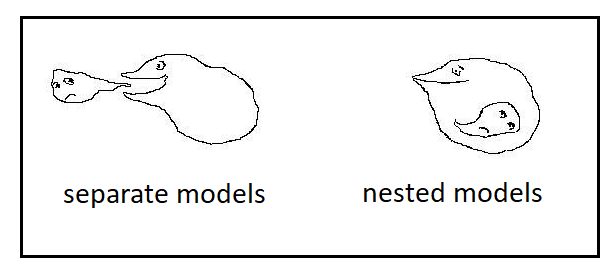
\includegraphics[width=0.5\textwidth]{images/AIC.png}
    \caption{Paveikslėlių numeriai rašomi apačioje, antraštė rašoma apačioje}
    \label{fig:grafikas1}
\end{figure}


Toliau eina tekstas po paveikslėliu.

\subsection{Sąrašai}

Nenumeruojamo sąrašo pavyzdys:
\begin{itemize}
    \item pirmasis elementas;
    \item antrasis elementas.
\end{itemize}

Numeruojamo sąrašo pavydzys:
\begin{enumerate}
    \item lorem ipsum dolor sit amet;
    \item consectetur adipiscing elit;
    \item vivamus a nisl gravida.
\end{enumerate}


\section{Programinio kodo pateikimas}
Šiame skyriuje pateikiamas programinio kodo pateikimo būdas rašto darbe.

\subsection{Algoritmai}

Algoritmai, lygiai taip pat, kaip ir paveikslėliai ar lentelės, yra numeruojami.
Juos būtina paminėti tekste, pvz.:~\ref{alg:gd} naudojamas surasti minimalią funkcijos $\mathcal{L}$ reikšmę.

\begin{algorithm}[h]
\caption{Gradientinio nusileidimo pseudokodas}\label{alg:gd}
\begin{algorithmic}[1]
    \STATE \textcolor{blue}{\texttt{\textbf{\# Darome prielaidą, kad $\mathcal{L}$ apibrėžtas tekste}}}
        \STATE Įeitis: $\mathcal{D}$ -- duomenų rinkinys
        \STATE Įeitis: $\theta_0$ -- parametrų atsitiktinių reikšmių inicializavimas
        \STATE Įeitis: $\gamma$ -- žingsnio dydis, mokymosi greitis (angl.~\textit{learning rate}, \textit{step size})
        \STATE Įeitis: $m$ -- epochų skaičius
        \FOR{$i = 1, 2, \dots, m$}
            \STATE $\theta_i \coloneq \theta_{i-1} - \gamma \nabla_\theta \mathcal{L}(\mathcal{D}, \theta_{i-1})$
            \STATE \textcolor{blue}{\texttt{\textbf{\# Funkcijos $\mathcal{L}$ išvestinė suskaičiuojama automatiškai, autograd pagalba}}}
        \ENDFOR
\end{algorithmic}
\end{algorithm}

\subsubsection{Skyrelio pavyzdys}
\noindent Nebūtina naudoti daug skyrelių (\textit{subsubsections}).

\sectionnonum{Rezultatai ir išvados}
Detaliau, kas turi būti parašyta šiame skyriuje, rasite atitinkamos programos metodiniuose reikalavimuose. 

\printbibliography[title = {Literatūra ir šaltiniai}]


\appendix
\renewcommand{\thesection}{\arabic{section} priedas.}

\section{\phantom{Priedas} Citavimo pavyzdžiai}
Dokumente - \textit{bibliografija.bib}, reikia sudėti visus cituojamus šaltinius ir panaudojus funkciją \textit{\{\textbackslash cite\{cituojamo objekto pavadinimas\}\}} atitinkamas šaltinis bus pridėtas prie literatūros šaltinių sąrašo.


\textit{bibliografija.bib} galima rasti kelių dažniausiai cituojamų šaltinių tipų pavyzdžius:
\begin{itemize}
    \item internetiniai puslapiai (\textit{@online}) \cite{PvzInternetinisPuslapis},
    \item duomenų rinkiniai (\textit{@dataset}) \cite{dataset}
    \item straipsniai (\textit{@article}) \cite{PvzStraipsnLt, PvzStraipsnEn}, 
    \item straipsniai iš konferencijos (\textit{@inproceedings}) \cite{PvzKonfLt, PvzKonfEn}, 
    \item knygos (\textit{@book}) \cite{PvzKnygLt, PvzKnygEn}, 
    \item baigiamieji darbai (\textit{@thesis arba mastersthesis/phdthesis} \cite{PvzMagistrLt, PvzPhdEn})
    \item elektroninės publikacijos (\textit{@misc}) \cite{PvzElPubLt, PvzElPubEn}
\end{itemize}

Taip pat yra pateikti pavyzdžiai - ChatGPT citavimui, tiek bendrai\cite{chatgpt_bendrai}, tiek konkrečiam pokalbiui\cite{chatgpt_pokalbis}.

\end{document}
